% Copyright 2004 by Till Tantau <tantau@users.sourceforge.net>.
%
% In principle, this file can be redistributed and/or modified under
% the terms of the GNU Public License, version 2.
%
% However, this file is supposed to be a template to be modified
% for your own needs. For this reason, if you use this file as a
% template and not specifically distribute it as part of a another
% package/program, I grant the extra permission to freely copy and
% modify this file as you see fit and even to delete this copyright
% notice. 

\documentclass{beamer}

% There are many different themes available for Beamer. A comprehensive
% list with examples is given here:
% http://deic.uab.es/~iblanes/beamer_gallery/index_by_theme.html
% You can uncomment the themes below if you would like to use a different
% one:
%\usetheme{AnnArbor}
%\usetheme{Antibes}
%\usetheme{Bergen}
%\usetheme{Berkeley}
%\usetheme{Berlin}
%\usetheme{Boadilla}
%\usetheme{boxes}
%\usetheme{CambridgeUS}
%\usetheme{Copenhagen}
%\usetheme{Darmstadt}
%\usetheme{default}
%\usetheme{Frankfurt}
%\usetheme{Goettingen}
%\usetheme{Hannover}
%\usetheme{Ilmenau}
%\usetheme{JuanLesPins}
%\usetheme{Luebeck}
\usetheme{Madrid}
%\usetheme{Malmoe}
%\usetheme{Marburg}
%\usetheme{Montpellier}
%\usetheme{PaloAlto}
%\usetheme{Pittsburgh}
%\usetheme{Rochester}
%\usetheme{Singapore}
%\usetheme{Szeged}
%\usetheme{Warsaw}


% Customize Warsaw color 
\setbeamercolor*{palette primary}{use=structure,fg=white,bg=red!50!black}
\setbeamercolor*{palette secondary}{use=structure,fg=white,bg=red!60!black}
\setbeamercolor*{palette tertiary}{use=structure,fg=white,bg=red!70!black}

% Customize Warsaw block title and background colors
\setbeamercolor{block title}{bg=red!50!black,fg=white}


% List your packages here

\usepackage[colorinlistoftodos]{todonotes}


\title[Progress Update]{Universal Platform for Building Energy Management}

% % A subtitle is optional and this may be deleted
% \subtitle{Product Proposal}

\author[B.~Lauer]{Brian~Lauer \\\and
Advisor: Dr. Suruz Miah}
% - Give the names in the same order as the appear in the paper.
% - Use the \inst{?} command only if the authors have different
%   affiliation.

\institute[Bradley University] % (optional, but mostly needed)
{
  Department of Electrical and Computer Engineering\\
  Bradley University\\
  1501 W. Bradley Avenue\\
  Peoria, IL, 61625, USA
}
% - Use the \inst command only if there are several affiliations.
% - Keep it simple, no one is interested in your street address.

\date[November~8,~2019]{Friday, November~8,~2019}
% - Either use conference name or its abbreviation.
% - Not really informative to the audience, more for people (including
%   yourself) who are reading the slides online

\logo{\hfill\href{http://www.bradley.edu}{
\includegraphics[width=0.75cm]{../figs/logoBU1-Print}}}  % place logo in every page 


\subject{Mobile Robot Localization}
% This is only inserted into the PDF information catalog. Can be left
% out. 

% If you have a file called "university-logo-filename.xxx", where xxx
% is a graphic format that can be processed by latex or pdflatex,
% resp., then you can add a logo as follows:

% \pgfdeclareimage[height=0.5cm]{university-logo}{university-logo-filename}
% \logo{\pgfuseimage{university-logo}}

% Let's get started
\begin{document}

\begin{frame}
  \titlepage
\end{frame}

\begin{frame}{Outline}
  \tableofcontents
  % You might wish to add the option [pausesections]
\end{frame}

% Section and subsections will appear in the presentation overview
% and table of contents.
\section{Objective}
\begin{frame}{Objective}
\begin{itemize}
\item Research and decide on a new device 
\end{itemize}
\end{frame}

\section{Stepper Motor}
\begin{frame}{Stepper Motor}
\begin{itemize}
\item Decided on stepping motor as new device
\item 28BYJ-48 with ULN2003A stepping motor driver
\begin{figure}
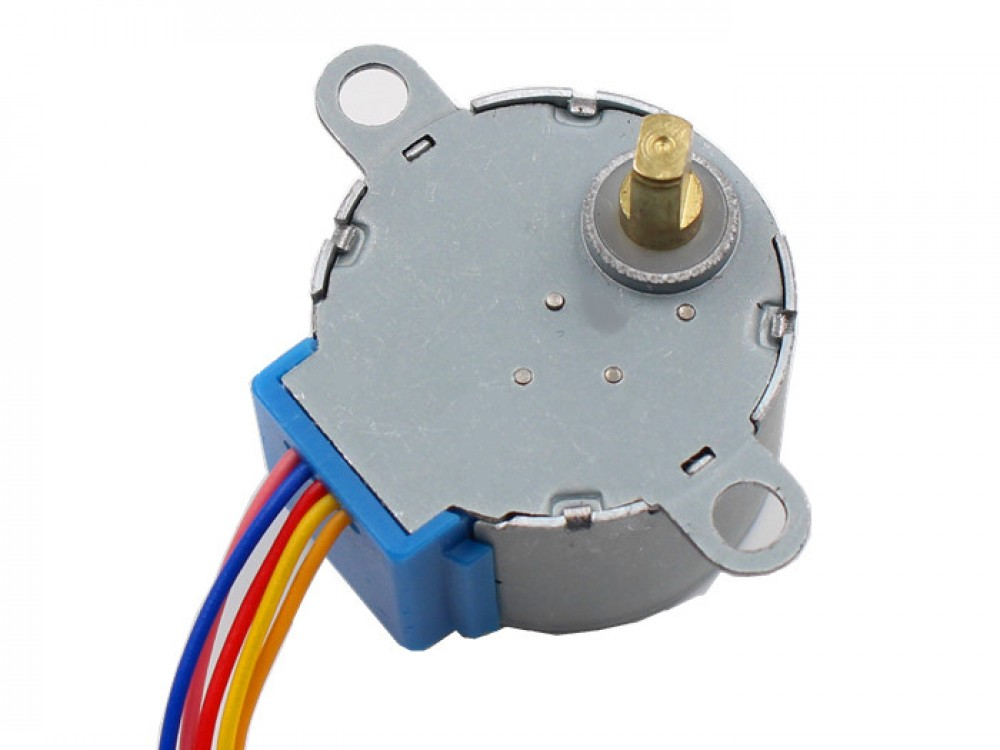
\includegraphics[scale=0.08]{../figs/28byj48stepper}
\caption{https://www.makerfabs.com/28byj-48-stepper-motor-5v.html}
\end{figure}

\begin{figure}
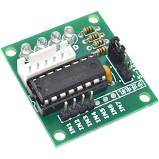
\includegraphics[scale=0.4]{../figs/uln2003astepper}
\caption{Aliexpress.com}
\end{figure}
\end{itemize}
\end{frame}

\section{Progress}
\begin{frame}{Progress}
\begin{figure}
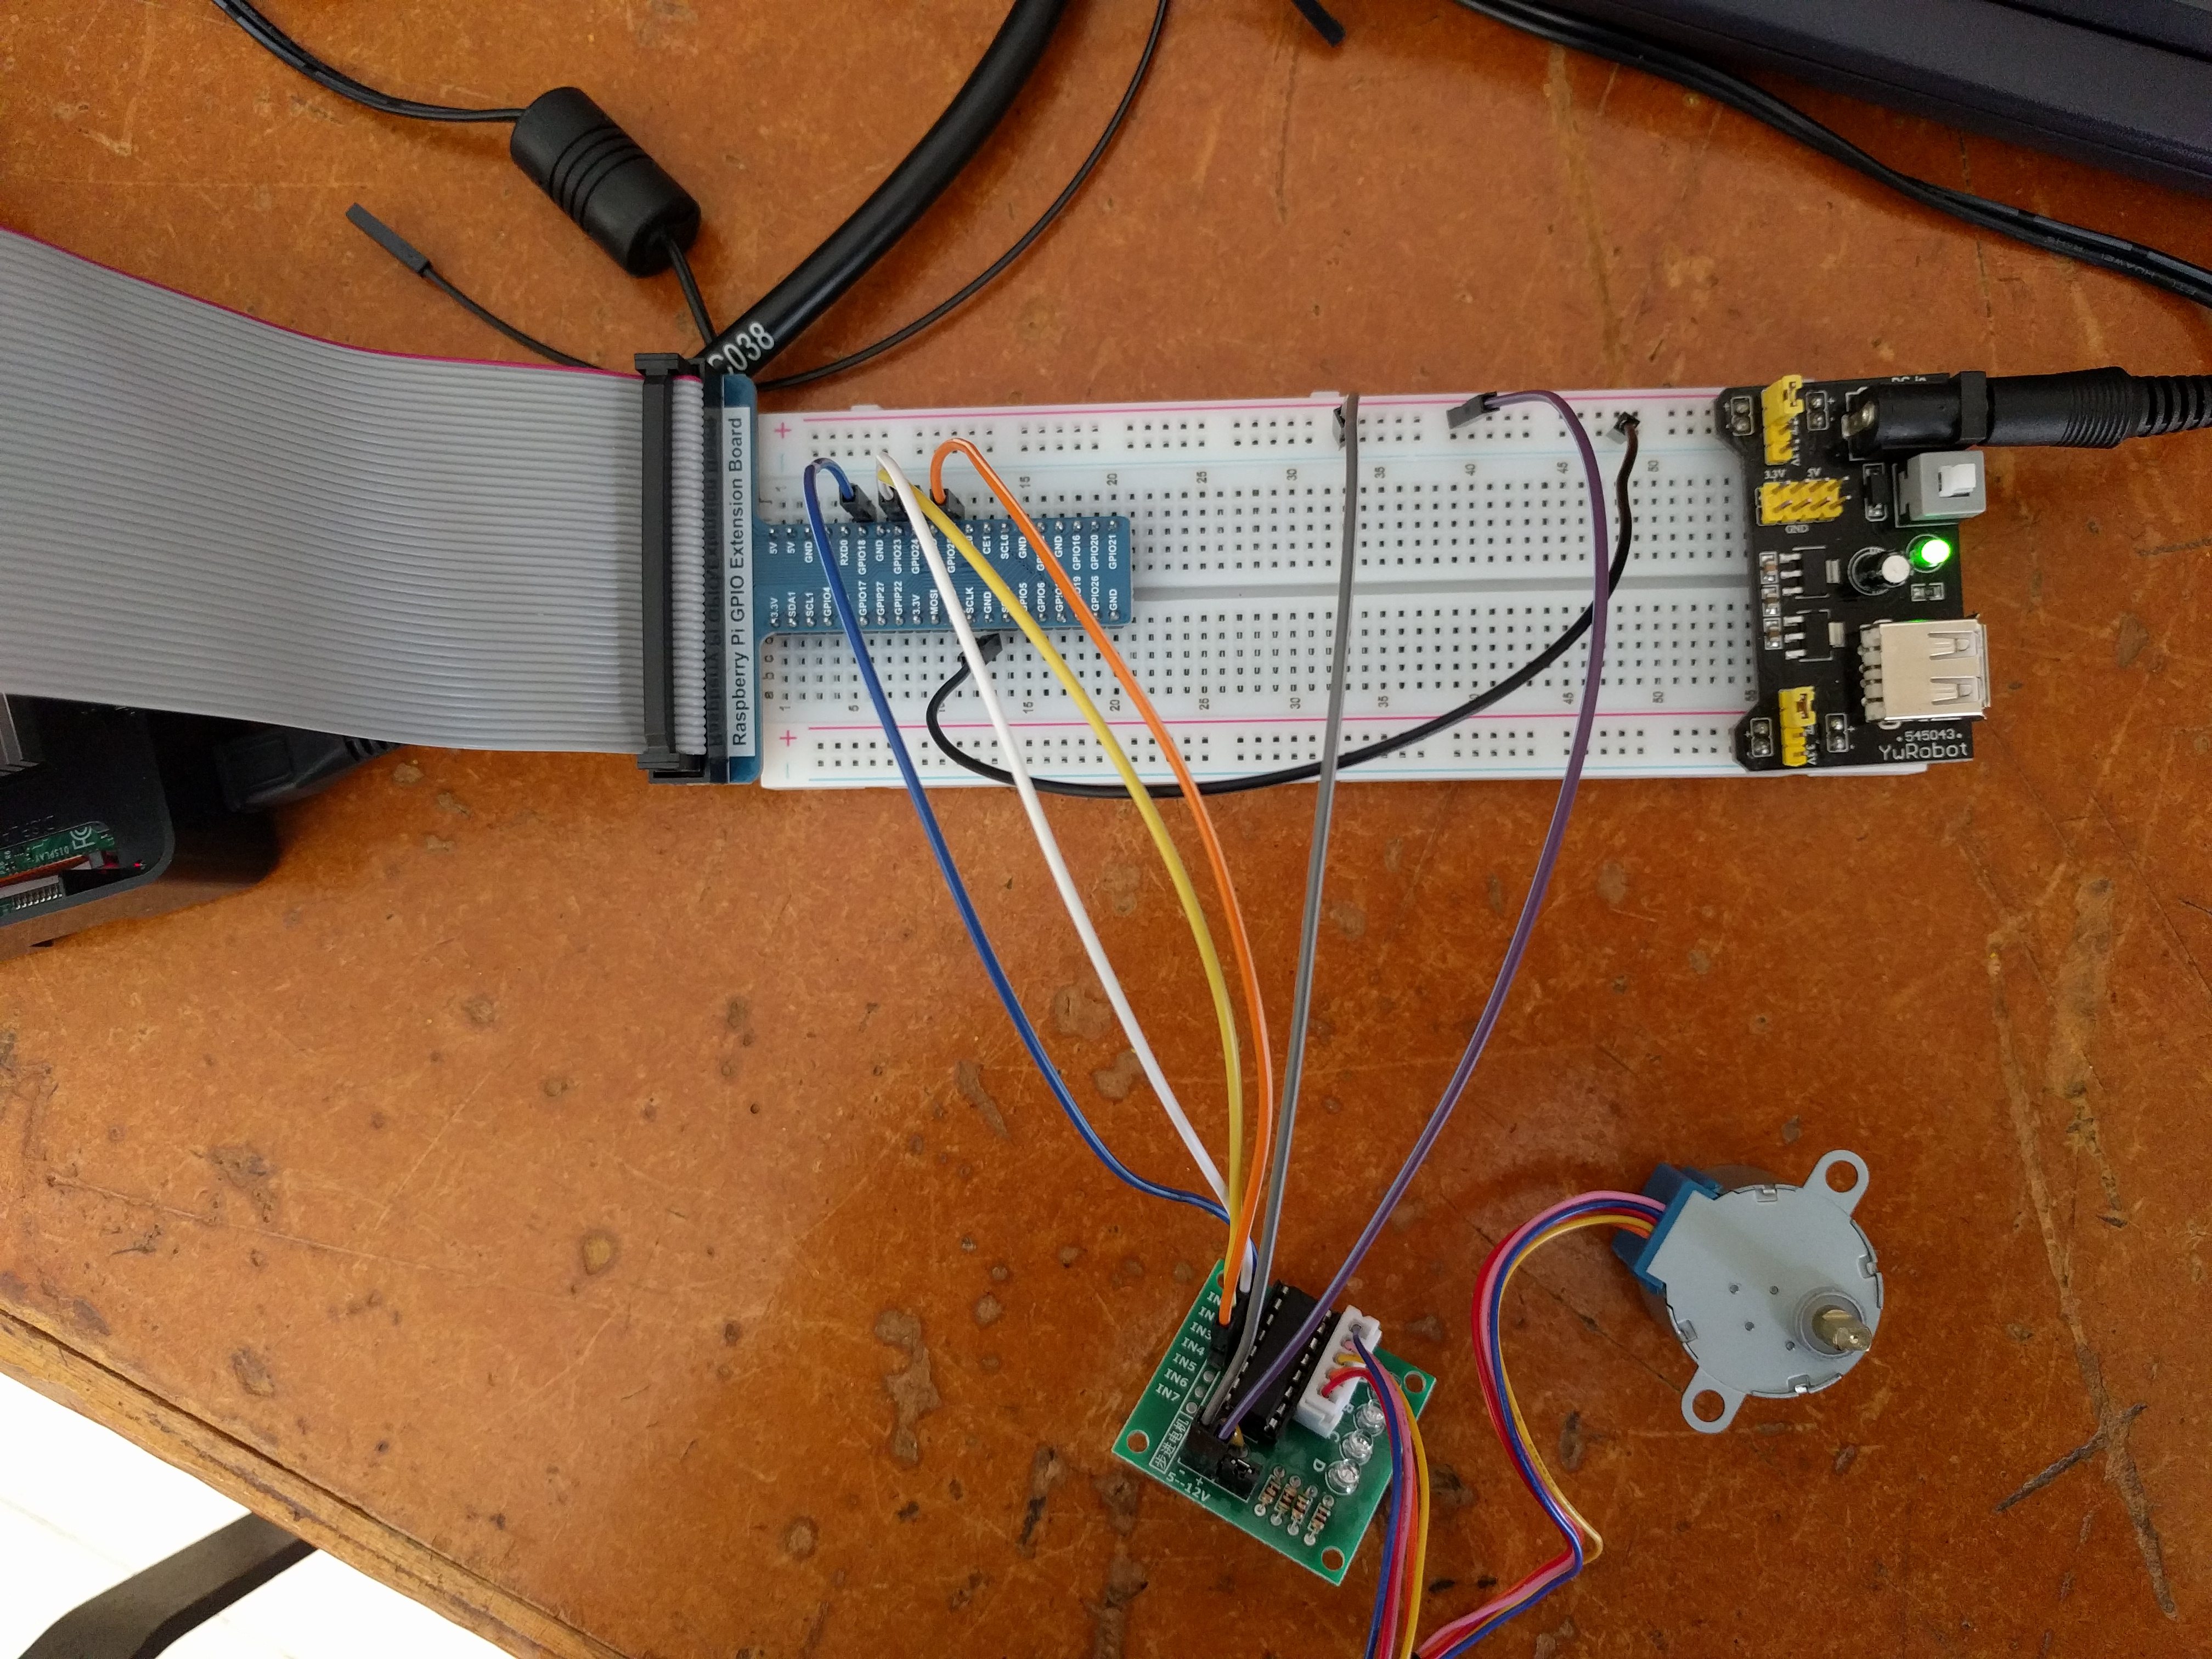
\includegraphics[scale=0.05]{../figs/labStepper}
\end{figure}
\end{frame}

\begin{frame}{Progress}
\begin{figure}
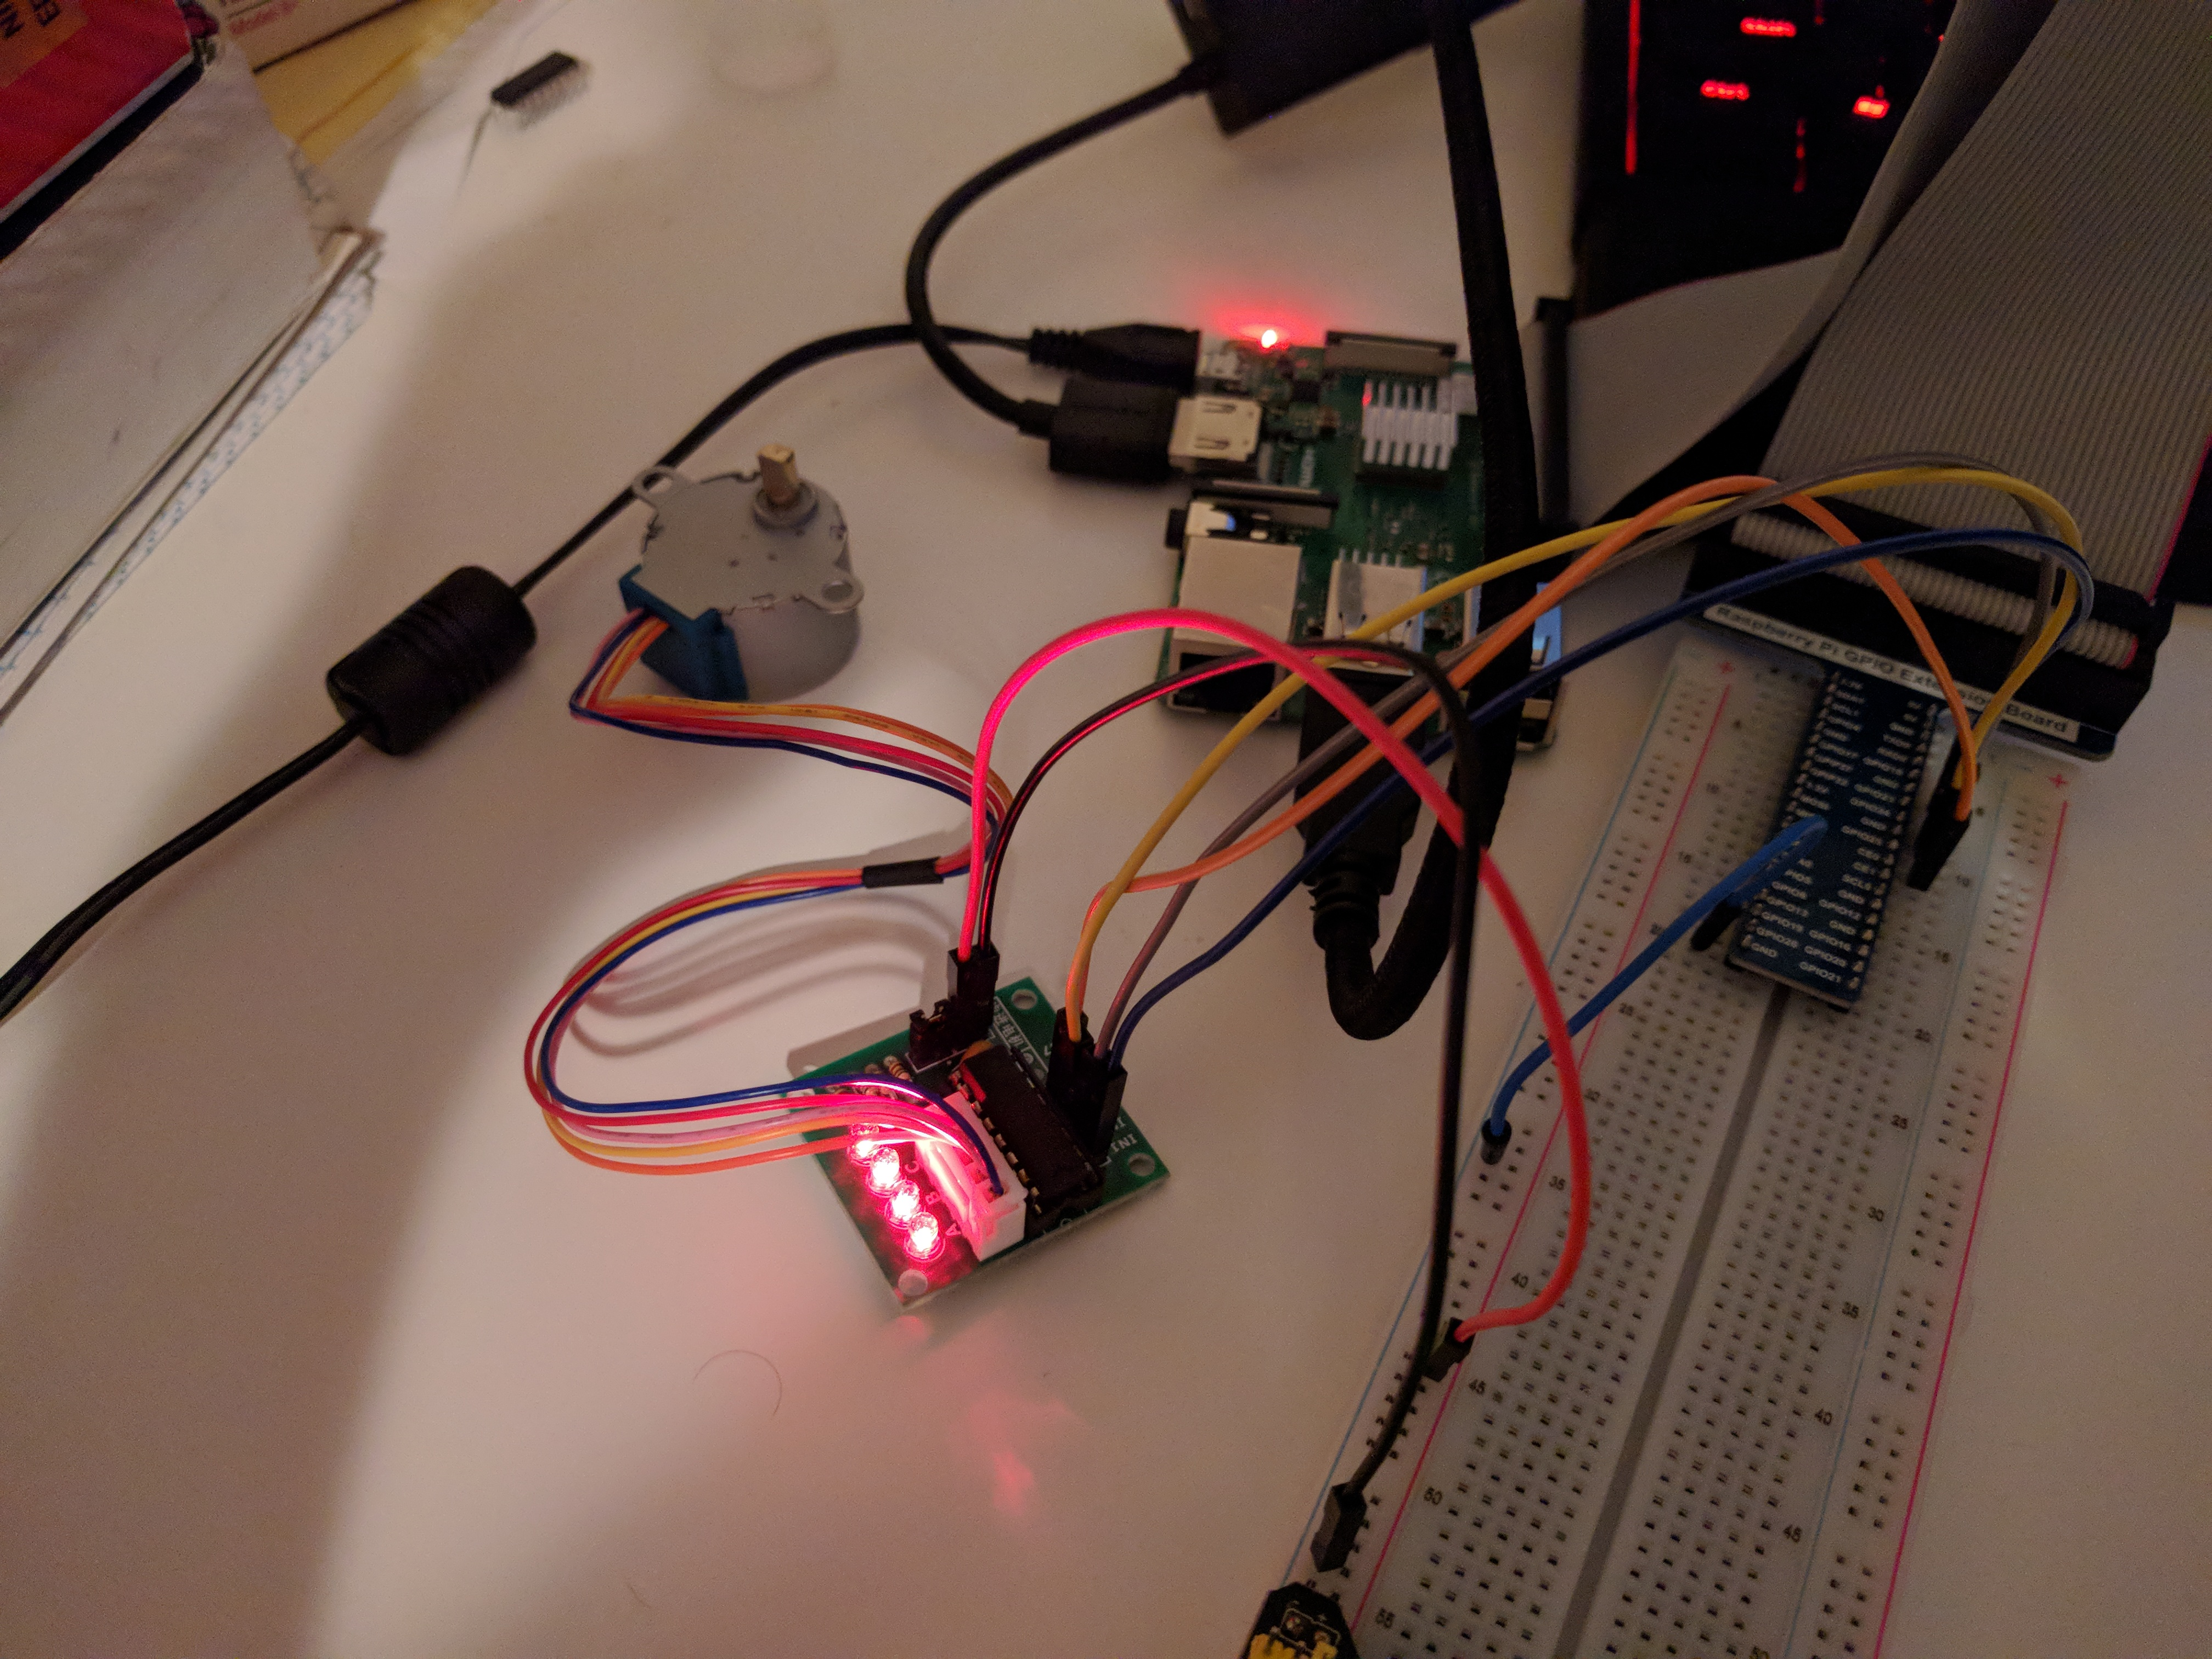
\includegraphics[scale=0.05]{../figs/homeStepperMotor}
\end{figure}
\end{frame}

\section{Plans}
\begin{frame}{Plans}
\begin{itemize}
\item Decide on whether to use XBee or Raspberry Pi to control motor
\item Create primitive TCP/IP web server on RPi using Python socket programming
\item Create widgets in device dashboard page for controlling motor (number of steps, run continuously)
\end{itemize}
\end{frame}
% All of the following is optional and typically not needed. 


% All of the following is optional and typically not needed. 
\appendix
\section<presentation>*{\appendixname}
\subsection<presentation>*{For Further Reading}

\begin{frame}[allowframebreaks]
  \frametitle<presentation>{For Further Reading}
    
  \begin{thebibliography}{10}
    
  \beamertemplatearticlebibitems
  % Followed by interesting articles. Keep the list short. 

  \bibitem{Someone2000}
    X. Zhang, R. Adhikari, M. Pipattanasomporn, M. Kuzlu, and S. Raihman
    \newblock Deploying IoT Devices to Make Buildings Smart:
Performance Evaluation and Deployment Experience.
    \newblock {\em 2016 IEEE 3RD World Forum on IOT}
  \end{thebibliography}
\end{frame}


\end{document}
\end{document}



%%% Local Variables:
%%% mode: latex
%%% TeX-master: t
%%% End:
